\chapter{Implementation}
\section{Implementation of Web Application}
\subsection{Software Implementation}
To host the live streaming server we are making use of the python script in the \\*back-end, communicating with the rendered front-end on the client side.\\
\newline
For the script we are using open-cv modules for support streaming and control of the stream parameters. 

\subsection{Hardware Implementation}
Raspberry Pi camera is used directly with the camera port on the Raspberry Pi.
\section{Implementation of Robot Movement}
\subsection{Software Implementation}

First the keystrokes are recorded using keyboard module in the form of a character, the recorded characters are then sent from server to client using TCP/IP sockets.\\
\newline
Upon receiving the character on the receiver side the appropriate action is \\*implemented using an if-else ladder which is reflected by the motion of the robot.
\newpage
\subsection{Hardware Implementation}
Raspberry Pi GPIO used in Board mode and is connected to the motor driver in the format given below:
\begin{enumerate}[ ]
\item Pin 13 – IN1(Left)
\item Pin 15 – IN2(Left)
\item Pin 16 – IN3(Right)
\item Pin 18 – IN4(Right)
\item Pin 32 – ENA(PWM - Left)
\item Pin 33 – ENB(PWM -Right)
\end{enumerate}
\begin{figure}[h]
\centering
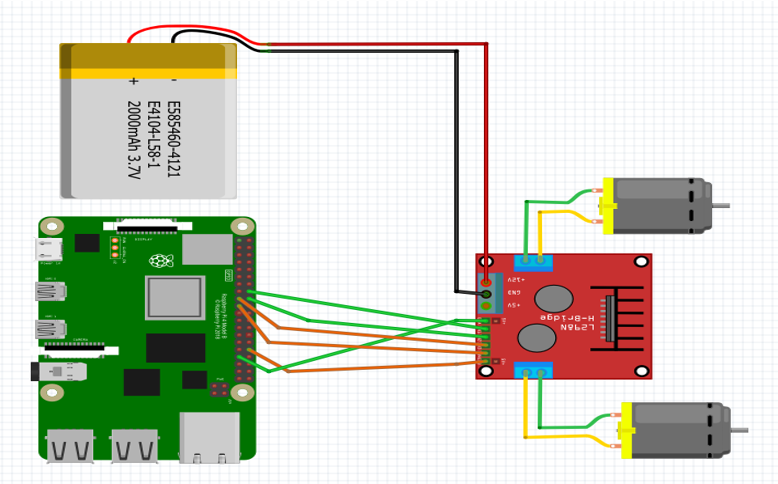
\includegraphics[scale=0.8]{ckt.png}
\caption{Circuit Connections}
\end{figure}